\begin{figure}
\pgfplotsset{every x tick label/.append style={font=\tiny, rotate=30}}
\pgfplotsset{every y tick label/.append style={font=\tiny}}
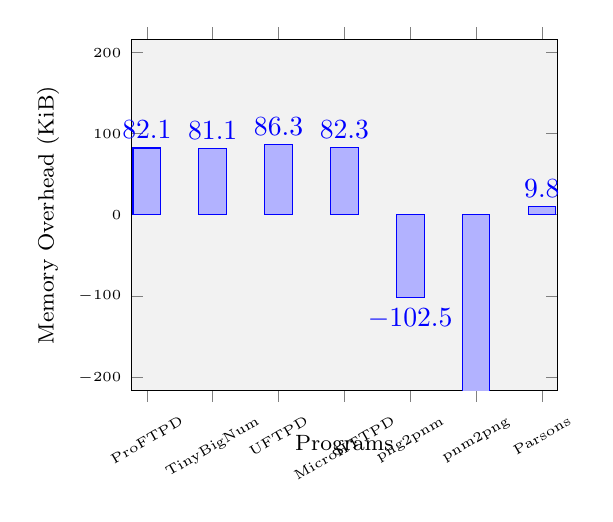
\begin{tikzpicture}  
  
\begin{axis}  
[  
    ybar,  
    ymin=-200, ymax=+200,
    enlargelimits=0.04,  
    ylabel={Memory Overhead (KiB)}, % the ylabel must precede a # symbol.  
    %xlabel={Programs},  
    symbolic x coords={ProFTPD, TinyBigNum, UFTPD, MicroHTTPD, png2pnm, pnm2png, Parsons}, % these are the specification of coordinates on the x-axis.  
    xtick=data,  
    bar width=10pt,
    width=7cm,
    x tick label/.append style={font=\tiny, rotate=30},
    y tick label/.append style={font=\tiny},
    axis background/.style={fill=gray!10},
    x label style={at={(axis description cs:0.5,-0.1)},anchor=north, font=\footnotesize},
    xlabel={Programs},
    ylabel style={font=\footnotesize},
     nodes near coords, % this command is used to mention the y-axis points on the top of the particular bar.  
    nodes near coords align={vertical},  
    ]  
\addplot coordinates {(ProFTPD,82.1) (TinyBigNum,81.1) (UFTPD, 86.3) (MicroHTTPD,82.3) (png2pnm, -102.5) (pnm2png, -51000) (Parsons, 9.8)};  
  
\end{axis}  
\end{tikzpicture} 
\caption{Memory Overhead of Partioned Programs.}
\label{fig:memoryoverhead}
\end{figure}
